\documentclass{article}
\usepackage[a4paper, portrait, margin=1in]{geometry}
\usepackage{graphicx}
\usepackage{array}
\usepackage{listings}
\usepackage{xcolor}
\usepackage[utf8]{inputenc}
\usepackage{blindtext}
\usepackage[export]{adjustbox}
\usepackage{enumerate}
\usepackage{amsmath}
\usepackage[skip=0.5ex]{subcaption}
\usepackage{caption}
\usepackage{lipsum}
\usepackage{tabularx}
\usepackage{makecell}

\definecolor{codegreen}{rgb}{0,0.6,0}
\definecolor{codegray}{rgb}{0.5,0.5,0.5}
\definecolor{codepurple}{rgb}{0.58,0,0.82}
\definecolor{backcolour}{rgb}{0.95,0.95,0.92}

\newtheorem{theorem}{Theorem}

\lstdefinestyle{mystyle}{
    backgroundcolor=\color{backcolour},
    commentstyle=\color{codegreen},
    keywordstyle=\color{magenta},
    numberstyle=\tiny\color{codegray},
    stringstyle=\color{codepurple},
    breakatwhitespace=false,
    breaklines=true,
    captionpos=b,
    keepspaces=true,
    numbers=left,
    numbersep=5pt,
    showspaces=false,
    showstringspaces=false,
    showtabs=false,
    tabsize=4
}



\begin{document}

\title{Student Id: 9910821}
\date{}

\maketitle
\section*{Introduction}
This report is a two part study of:
\begin{enumerate}[I)]
  \item Montecarlo techniques used to value a portfolio of european, path independent options.
  Extensions of this method such as antithetic variables and moment-matching were also investigated vis-a-vis confidence intervals and variance reduction.
  \item Montecarlo techniques (and extensions) used to value a discrete, fixed-strike Asian call option
  which is an example of a path dependent option. Particular study is also carried out on computational processing time required and
  algorithm efficiency.
\end{enumerate}

\section*{Task 1}
This task consisted in valuing a portfolio comprising of shorting a call option with strike price $X_1$,
 longing a call option with strike price $X_2$, longing $2 X_2$ binary cash or nothing call options with strike
 price $X_2$ and unit payoff and longing a call option with strike price equal to zero with parameters:

\begin{flushleft}
$T$=0.5, $\sigma$=0.41, $r$=0.03, $D_0$=0.04, $X_1$=70.0 and $X_2$=100.0.
\end{flushleft}
Montecarlo methods of estimation have at their core the law of large numbers which states that for a number $N$ of
trials tending to infinity, the average of all the observations tends to the expected value. Formally,
\begin{theorem}
The sample average $\overline{X}$ converges almost surely to the expected value $\mu$.
$\overline{X}_n \to \mu$ for $ n \to \infty$
\label{thrm:LLN}
\end{theorem}
Hence, Montecarlo methods are a technique in which a large quantity of randomly generated numbers (usually denoted by $N$) are
studied using a probabilistic model to find an approximate solution to a
numerical problem that would be difficult to solve by other methods.
\\
\subsection*{Analytic Values}
Before attempting numerical methods of solving the valuation of the portfolio it is important we have a value
to check our results with. Luckily there are analytic solutions to the different options in the portfolio currently being
analysed and these combine to produce our final value of $V(S_0,t=0)$. The following represent the analytic formulae used:
\begin{enumerate}[I)]
  \item A call option with value of underlying $S$ at time $t$, strike price $X$ at maturity $T$ and interest rate $r$:
  \begin{equation}
    C(S,t)=Se^{-D_0(T-t)}N(d_1)-Xe^{-r(T-t)}N(d_2)
    \label{eq:analytic1}
  \end{equation}
  \item A binary call option with unit payoff at maturity T:
  \begin{equation}
    BC(S,t)=e^{-r(T-t)}N(d_2)
     \label{eq:analytic2}
  \end{equation}
\end{enumerate}
  The values $d_1$ and $d_2$ are variables calculated from the other parameters with formulae:
  \begin{equation}
    d_1= \frac{\ln(\frac{S}{X})+(r-D_0+\frac{1}{2}\sigma^{2})}{\sigma\sqrt{T-t}}
     \label{eq:analytic3}
  \end{equation}
  and
  \begin{equation}
     d_2= d_1- \sigma\sqrt{T-t}
      \label{eq:analytic4}
  \end{equation}
\begin{figure}[!th]
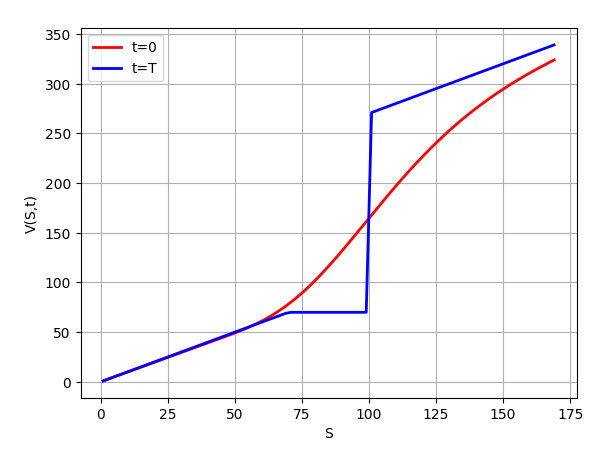
\includegraphics[width=0.7\textwidth,center]{analytic_values.png}
\caption{Plots of the price of the portfolio at times $t=0$ and $t=T$ using analytic solutions.}
\label{fig:analytic_values}
\end{figure}
Figure \ref{fig:analytic_values} illustrates the value of the portfolio calculated using the analytic Formulae \ref{eq:analytic1} to \ref{eq:analytic4}. We are particularly interested in the $t=0$ case since we will be checking the estimators used later on with these values to measure accuracy.
\subsection*{Analysing Montecarlo Methods}
The first and most basic method of estimation attempted in this report was the 'normal' Montecarlo method.
For a particular path $m$ (where $m$ runs from 1 to $M$) , a random number is generated from a pseudorandom number generator (PRNG) of choice $N$ times. In this case, a Mersenne Twister was chosen which is based on the Mersenne prime $2^{19937}-1$. This particular PRNG was chosen as it has very long periods, passes most statistical tests for randomness and has fast random number generation. The price of the stock is let to fluctuate and the average value after $N$ fluctuations is taken. From Theorem \ref{thrm:LLN} we expect the value of the portfolio to tend to the analytic value as $N$ tends to a very large number. The results for this method are shown in Table \ref{table:normal_mc}.
\begin{table}[h!]
\centering
\begin{tabularx}{\textwidth}{c|c c c c}
  \makecell{$N$\\(thousands)} & $ V(S_0=X_1,t=0)_{MC} $ & $ V(S_0=X_1,t=0)_A$ & $ V(S_0=X_2,t=0)_{MC} $ & $ V(S_0=X_2,t=0)_A$ \\
 \hline
1 & 77.8243 & 78.1939 &  164.73  &  164.564\\
2 & 78.3079 & 78.1939 &  164.662  &  164.564\\
5 & 78.1757 & 78.1939 &  164.694  &  164.564\\
10 & 78.1372 & 78.1939 &  164.546  &  164.564\\
50 & 78.2078 & 78.1939 &  164.615  &  164.564\\
100 & 78.1909 & 78.1939 &  164.615  &  164.564\\
\end{tabularx}
\caption{A table showing Montecarlo (MC) estimated values for the portofolio $V(S_0,t=0)$ compared to the analytic value (A) for different values of Montecarlo iterations $N$.}
\label{table:normal_mc}
\end{table}
The Montecarlo estimate value for the portfolio does indeed tend to analytic value which is a good sign that this estimator works. However careful attention must be paid to what confidence one can put on such method and its results. A few good metrics for this are the variance (or sample variance) and confidence intervals. In the next subsection we analyze more in detail the confidence in the results of this methods and investigate possible extensions to this which make thus confidence better.
\pagebreak
\subsection*{Accuracy and Confidence Intervals}
A corollary of Theorem \ref{thrm:LLN} is that, assuming finite variance
\begin{equation}
  {Var} (X_{i})=\sigma ^{2} = \frac{\sum{X-\mu}^2}{M}
  \label{eq:oneVariance}
\end{equation}
for all $i$ and no correlation between random variables, the variance for the average value of $M$ paths of our Montecarlo sampling is given by
\begin{equation}
  Var(\overline {X}_{M}) = \frac {\sigma ^{2}}{M}
  \label{eq:variance}
\end{equation}
but since we are sampling a finite number of paths and not taking an infinite number of paths we use the sample variance given by
\begin{equation}
  Var(\overline {X}_{M}) = \frac {\sigma ^{2}}{M-1}.
  \label{eq:sampleVariance}
\end{equation}
Finally, we can use the Central Limit Theorem which states that when independent random variables are added, their properly normalized sum tends toward a normal distribution. For us it means we can relate the sample variance to the standard deviation which implies about 95\% confidence that repeated runs of the trial would result within 2 standard deviations of the mean. Applying these to the basic Montecarlo method explained previously produces the plot seen in Figure \ref{fig:confidence1}. The red envelope is the 95\% confidence level and one immediate observation is that this covers completely the results of the simulatiom. This mean that the variance is very high and our results are far from reliable.
\\
\\
Thus, there is a need for variance reducing methods which build upon Montecarlo. One such method is the use of \textbf{antithetic variables}. The idea is that instead of drawing only a normally distributed $\phi$ we now draw a pair $-\phi$ and add it to the sum and at the end divide by $2N$. The advantage of using this method is that the sum is ensured to be 0 as required and that variance be 1 ( by matching the mean and skewness to the required one,the variance is thus ensured). To keep everything comparable $\frac{N}{2}$ such numbers were drawn so the total remains $N$ as before. The results can be seen in Figure \ref{fig:confidence2}.
\\
\\
One further method investigated was \textbf{moment matching}. Similarly to antithetic variables, $\frac{N}{2}$ random numbers are sampled together with their pair. The total variance of these is calculated and then the whole set of numbers is divided element-wise by the square root of the variance. This ensures a variance of 1 as required. The  results can be seen in Figure \ref{fig:confidence3}.
\\
\begin{table}[h]
\centering
\begin{tabular}{c|c c c c}
 \makecell{$N$\\(thousands)} & $V_{MC}$ & $ V_{AV}$ & $V_{MM}$ & $V_A$ \\
 \hline
1 & 77.8243$\pm{20.637}$ & 78.163$\pm{15.9292}$ & 78.2931$\pm{10.1584}$  &  78.1939\\
2 & 78.3079$\pm{12.9237}$ & 78.1904$\pm{9.58466}$ &  78.26$\pm{6.21086}$  &  78.1939\\
5 & 78.1757$\pm{8.3882}$ & 78.2445$\pm{7.62567}$ &  78.2246$\pm{4.64797}$  &  78.1939\\
10 & 78.1372$\pm{5.30014}$ & 78.1608$\pm{5.31964}$ &  78.2444$\pm{2.63015}$  &  78.1939\\
50 & 78.2078$\pm{2.45959}$& 78.1939$\pm{2.62684}$ &  78.1851$\pm{1.57154}$  &  78.1939\\
100 & 78.1909$\pm{1.98767}$ & 78.1924$\pm{1.40195}$ &  78.2065$\pm{0.909534}$  &  78.1939\\
\end{tabular}
\caption{A table showing basic Montecarlo (MC) estimated values for the portofolio $V(S_0=X_1,t=0)$ compared to the antithetic variables (AV), moment matching (MM) and analytic (A) methods for different values of Montecarlo iterations $N$.}
\label{table:mc_comparisons}
\end{table}
\\
The results, shown in Figure \ref{fig:confidence} and compared in the Table \ref{table:mc_comparisons}, indicate a clear trend of increasing confidence and accuracy for the methods described.
Moment matching appears to be the best of these methods, precision-wise, achieving sub 2\% error on the mean.
Ensuring the mean and variance match the required ones from our assumptions of Gaussian noise means the results not only converge better toward the analytic value but the precision they carry with them increases.
\clearpage
\begin{figure}[!h]
\begin{minipage}{.5\textwidth}
  \centering
  \begin{subfigure}{\textwidth}
      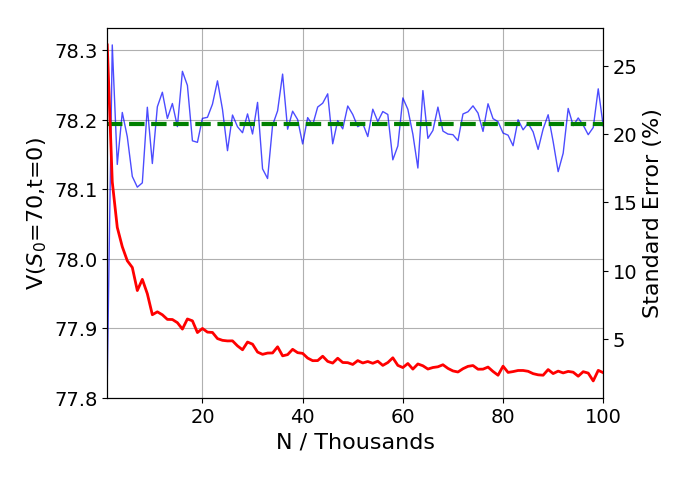
\includegraphics[width=\linewidth]{confidence_70_normal.png}
      \subcaption{Basic Montecarlo method with $S_0$=70}
      \label{fig:confidence1}
  \end{subfigure}
  \medskip
  \begin{subfigure}{\textwidth}
      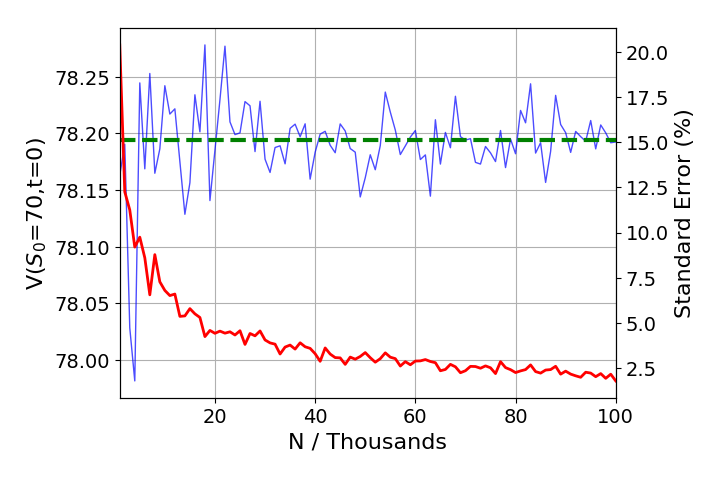
\includegraphics[width=\linewidth]{confidence_70_antithetic.png}
      \subcaption{Antithetic Variables method with $S_0$=70}
      \label{fig:confidence2}
  \end{subfigure}
  \medskip
  \begin{subfigure}{\textwidth}
      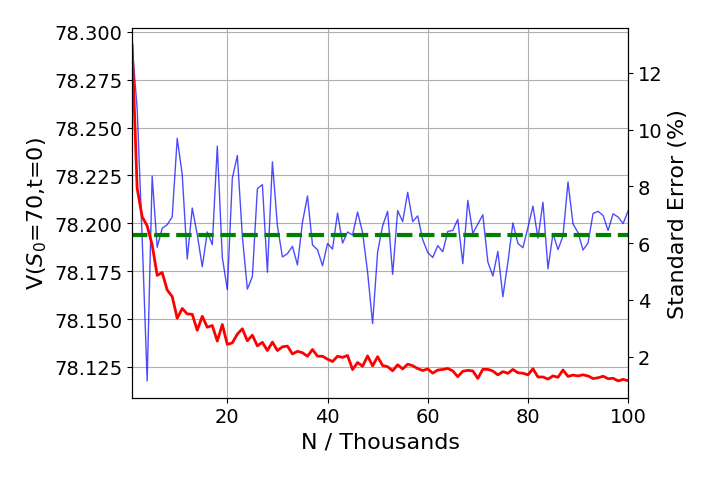
\includegraphics[width=\linewidth]{confidence_70_momentmatch.png}
      \subcaption{Moment Matching method with $S_0$=70}
      \label{fig:confidence3}
  \end{subfigure}
\end{minipage}
\begin{minipage}{.5\textwidth}

  \centering
  \begin{subfigure}{\textwidth}
      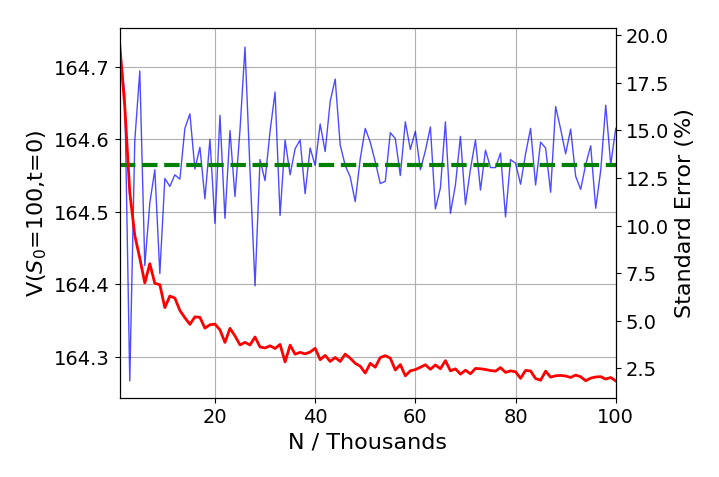
\includegraphics[width=\linewidth]{confidence_100_normal.png}
      \subcaption{Basic Montecarlo method with $S_0$=100}
      \label{fig:confidence1}
  \end{subfigure}
  \medskip
  \begin{subfigure}{\textwidth}
      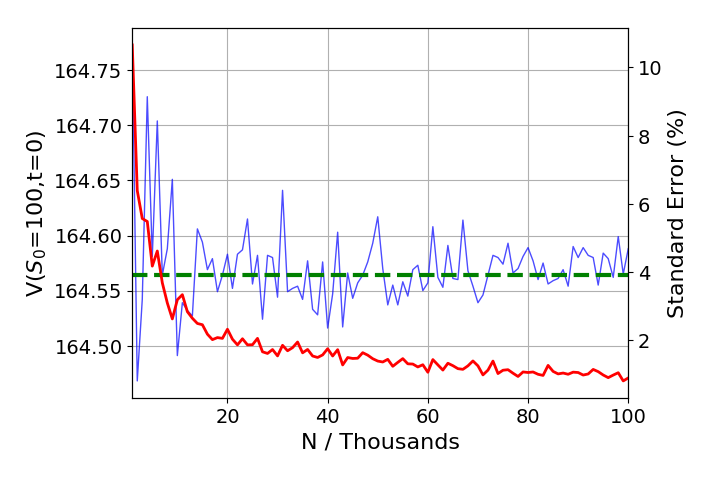
\includegraphics[width=\linewidth]{confidence_100_antithetic.png}
      \subcaption{Antithetic Variables method with $S_0$=100}
      \label{fig:confidence2}
  \end{subfigure}
  \medskip
  \begin{subfigure}{\textwidth}
      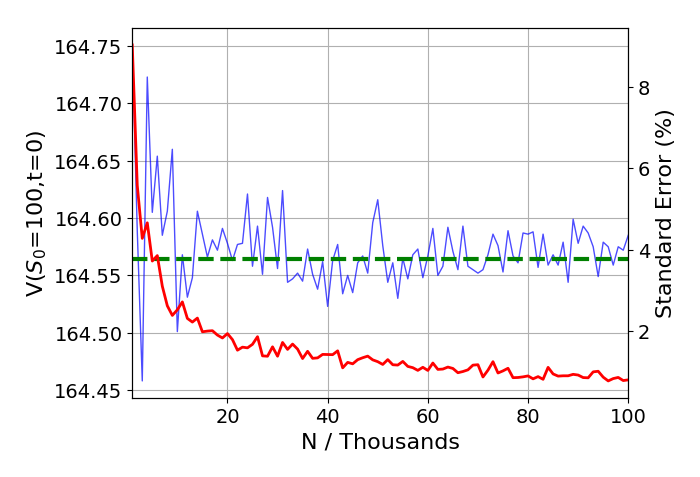
\includegraphics[width=\linewidth]{confidence_100_momentmatch.png}
      \subcaption{Moment Matching method with $S_0$=100}
      \label{fig:confidence3}
  \end{subfigure}
\end{minipage}

\includegraphics[width=\linewidth]{legend.png}
\caption{Plots of the price of the portfolio at time $t=0$ for $S_0 = X_1$ (a-c) and $S_0 = X_2$ (d-f) using normal (a,d), anithetic variable (b,e) and moment matching (c,f) methods respectively.}
\label{fig:confidence}
\end{figure}
\clearpage
\subsection*{Computational Efficiency}
One final remark should be made about the efficiency in processing time required by the three estimation methods described previously.
As described before, moment matching and antithetic variables require $\frac{N}{2}$ random numbers while basic Montecarlo requires $N$ which explains
the shapes of the curves in Figure \ref{fig:timing_efficiency}. The difference between moment matching and antithetic variables might be explained by the requirement of the former of one more for loop than the latter.
Due to the results in Figure \ref{fig:confidence} one can say that using moment matching is the best method since the relatively small increase in computing time required produces very precise and accurate results when compared to the analytic values.
\begin{figure}[!th]
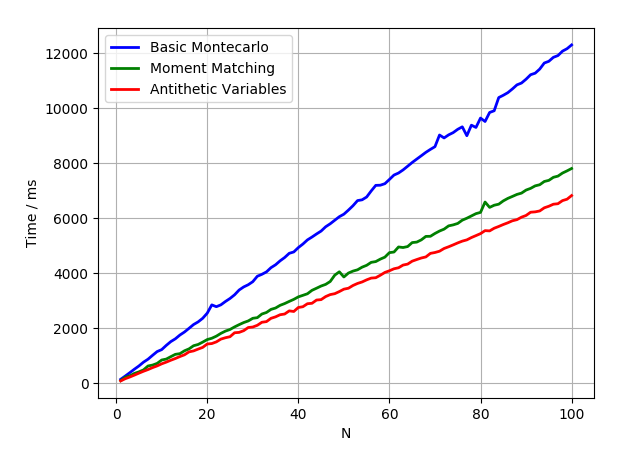
\includegraphics[width=0.7\textwidth,center]{timing_efficiency_100.png}
\caption{Plots of the time taken by the particular estimation method for $M=100$ paths as a function of Montecarlo random numbers generated $N$.}
\label{fig:timing_efficiency}
\end{figure}
\section*{Task 2}
This task consisted in valuing a discrete fixed-strike Asian call option with the following parameters:
\begin{flushleft}
$T$=2, $\sigma$=0.42, $r$=0.03, $D_0$=0.02, $X$=64000
\end{flushleft}
Due to the results shown in the previous task (Figure \ref{fig:confidence}), I decided to use antithetic paths to estimate this option thus using an efficient Montecarlo extension.
As before the method is the same when it comes to generating $N$ random numbers and fluctuating the stock using this parameter.
The difference in these options as the name implies is that since they are functions of the average of the price of the stock at some predetermined
time intervals, the path the stock takes changes the final result. Thus the method is to subdivide time from 0 to maturity in $K$+1 time steps and for a discrete fixed-strike Asian call option the 'floating' strike price is the average of sampling at $K+1$ intervals.
The natural first trend to investigate is the correlation (or lack) between the parameters $K$, $N$ and the value of the option.
\clearpage
\begin{table}[!h]
\centering
\begin{tabular}{c|c c c c}
 & & & \multicolumn{2}{c}{95 \% Confidence Levels} \\
\cline{4-5}
\makecell{$N$\\(thousands)} & K & $V_{MC}$ & Lower Level & Upper Level \\
\hline
1   & 20  & 8838.6 & 8712.99 & 8964.21      \\
50  & 20  & 8864.3 & 8847.72 & 8880.88     \\
100  & 20  & 8863.08&8849.54&8876.63      \\
1   & 50  & 8734.19&8624.81&8843.56      \\
50  & 50  & 8671.95&8656.07&8687.84       \\
100 & 50  & 8670.35&8659.22&8681.49       \\

\hline
\end{tabular}
\caption{Table showing antithetic paths extended Montecarlo (MC) estimated values for the option.
The number of paths is kept constant to $M$=50.}
\label{table:mc_comparisons}
\end{table}
The table highlights the most important trends, further pictorially illustrated by Figures \ref{fig:k_n} and Y.
\textbf{An increase in $K$ appears to decrease the value of the option}. This can be interpreted by remembering that $K+1$
is the number of intervals into which the time between 0 and maturity is set and by which the 'floating' strike value is
calculated. By taking more samples the option is more susceptible to volatility within those intervals. Having more intervals means
betting on a higher set of possible intervals which make up the final price against which the strike price is tested. Thus, with higher
volatility susceptibility come lower prices to account for it.

\begin{figure}[!bh]
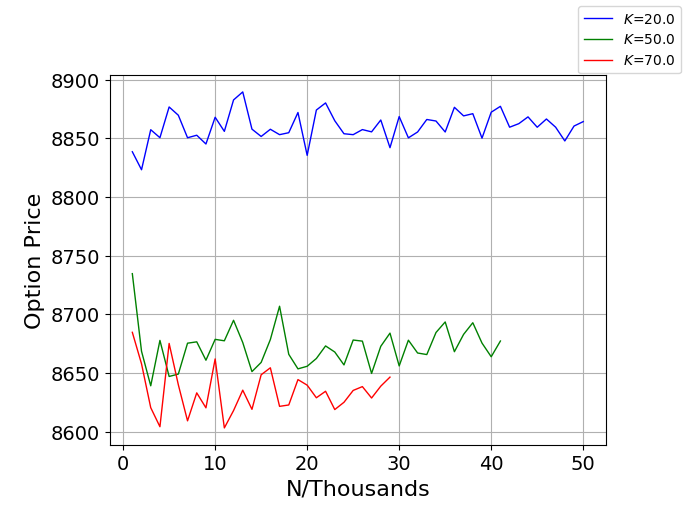
\includegraphics[width=0.7\textwidth,center]{task_2_2_plot_5.png}
\caption{Value of the option as a function of increasing $N$ for different values of $K$.
The number of paths is fixed to $M$=100. Larger $K$ values were stopped earlier when the simulation took $>30$s since the point was to observe trends in option value not time.}
\label{fig:k_n}
\end{figure}

\subsection*{Strict Timing}
The final part of this task was to obtain the most accurate value possible for the option using any Montecarlo method of choice, in this case antithetic paths, within 10 seconds of computation for a fixed $K=20$.
Figures \ref{fig:std_n} and \ref{fig:std_path} were plotted to understand which parameter between the number of paths $M$ and the number of random numbers generated $N$ was best to increase and focus on.
The vertical, purple dashed lines show the limit at which 10s of computation were exceeded.
Given these figures, I decided to compromise between number of paths and Montecarlo iterations to produce the final results in Table \ref{table:final}.
\begin{figure}[!h]
  \centering
  \begin{subfigure}{0.6\textwidth}
      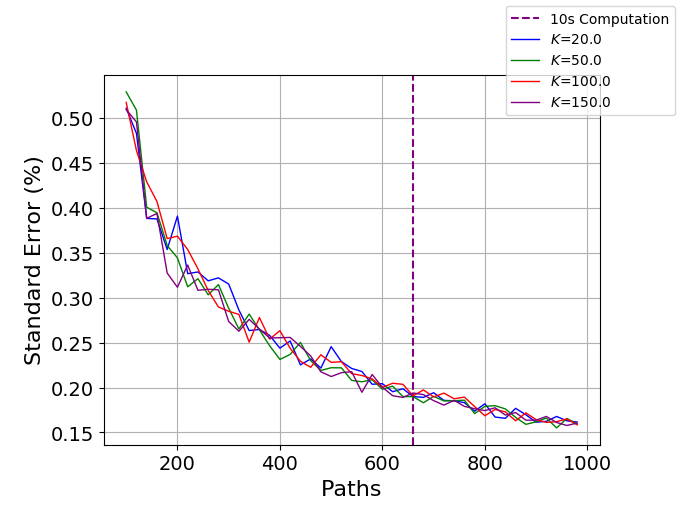
\includegraphics[width=\linewidth]{task_2_2_plot_2.png}
      \subcaption{Plot of the error on the mean value for the option for increasing number of paths $M$.
      The value of $N$ was fixed to 1000.}
      \label{fig:std_n}
  \end{subfigure}
  \medskip
  \begin{subfigure}{0.6\textwidth}
      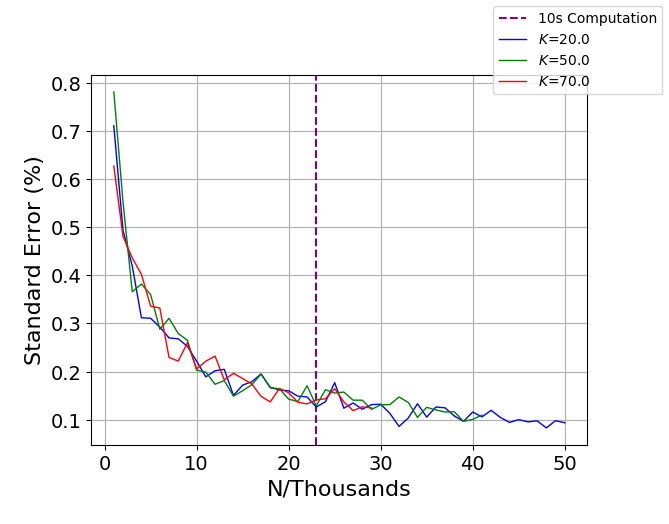
\includegraphics[width=\linewidth]{task_2_2_plot_6.png}
      \subcaption{Plot of the error on the mean value for the option for increasing number of Montecarlo loops $N$.
      The value of $M$ was fixed to 50.}
      \label{fig:std_path}
  \end{subfigure}
\caption{Plots of the error on the mean value for the option for increasing parameters $N$ and $M$.}
\label{fig:std_vars}
\end{figure}
\begin{table}[!h]
\centering
\begin{tabular}{c|c c c c c c}
 & & & & & \multicolumn{2}{c}{95 \% Confidence Levels} \\
\cline{6-7}
\makecell{$N$\\(thousands)} & K & M & Time(ms) &$V_{MC}$ & Lower Level & Upper Level \\
\hline
9000   & 20  & 300 & 9987 & 8857.54 & 8839.64 & 8875.45      \\
\hline
\end{tabular}
\caption{Table showing final result for antithetic paths extended Montecarlo (MC) estimated values for the option.}
\label{table:final}
\end{table}

\clearpage
\section*{Appendix}
\lstset{style=mystyle}
\subsection*{Portfolio Pricing Program Listing}
\lstinputlisting[language=C++]{../assignment_3.cpp}
\subsection*{Graphing Program Listing}
\lstinputlisting[language=Python]{../assignment_3.py}
\end{document}